\section{Preventivo}
	\subsection{Dettaglio attività}
		\textcolor{red}{assicurarsi che sia temrine giusto. cookies avevano messo "fase" ma tv li ha rektati}
		\subsubsection{Analisi dei Requisiti di Massima}
			\paragraph{Suddivisione lavoro} \Spazio
			Nell'attività di \textit{Analisi dei Requisiti di Massima} ciascun componente del gruppo andrà a rivestire i seguenti ruoli:
			\begin{table}[H]
				\centering
				\begin{tabular}{|C{4cm}|C{0.6cm}|C{0.6cm}|C{0.6cm}|C{0.6cm}|C{0.6cm}|C{0.6cm}|C{3cm}|}
					\hlineB{3}
				\thead{Nominativo} &\thead{Re} &\thead{Am} &\thead{An}&\thead{Pt}&\thead{Pr}&\thead{Ve}&\thead{Ore totali}\\
					\hlineB{3}
					Paolo Eccher        & -  & 3 & 13 & - & - & 6 & 22 \\
					Alberto Gallinaro   & -  & - & 16 & - & - & 6 & 22 \\
					Giuseppe Merlino    & 13 & - & 2 & - & - & 7 & 22 \\
					Elia Montecchio     & -  & 3 & 12 & - & - & 6 & 21 \\
					Lisa Parma          & -  & 6 & 12 & - & - & 4 & 22 \\
					Francesco Parolini  & 13 & 4 & - & - & - & 6 & 23 \\
					Davide Zago         & 5  & 2 & 10 & - & - & 6 & 23 \\
					\textbf{Ore totali ruolo}  & \textbf{31} & \textbf{18} & \textbf{65} & \textbf{-} & \textbf{-} & \textbf{41} & \textbf{155} \\
					\hlineB{3}
				\end{tabular}
				\caption{Suddivisione del lavoro - \textit{Analisi dei Requisiti di Massima}}	
			\end{table}
			
			Tali dati sono riassunti graficamente nel seguente diagramma a barre:
			
			\textcolor{red}{METTERE DIAGRAMAM}		
			
			\paragraph{Prospetto economico} \Spazio
			Nello svolgimento di questa attività i costi sostenuti per ogni ruolo, non a carico del proponente trattandosi dell'investimento iniziale, sono riassunti nella seguente tabella:
			\begin{table}[H]
				\centering
				\begin{tabular}{|p{4cm}|C{4cm}|C{4cm}|}
					\hlineB{3}
					
					\thead{Ruolo} &\thead{Ore previste} &\thead{Costo}\\
					
					\hlineB{3}
					Responsabile & 31 & 930,00\euro \\
					\hline
					Amministratore& 18 & 360,00\euro \\
					\hline
					Analista & 65 & 1.625,00\euro \\
					\hline
					Progettista & - & 0\euro \\
					\hline
					Programmatore & - & 0\euro \\
					\hline
					Verificatore & 41 & 615,00\euro \\
					\hline				
					\textbf{Ore totali} & \textbf{155} & \textbf{3.530.00 \euro} \\
					\hlineB{3}
				\end{tabular}
				\caption{Costi per ruolo - \textit{Analisi dei Requisiti di Massima}}
			\end{table}

			
			La suddivisione delle ore di lavoro tra i vari ruoli è raffigurata graficamente attraverso il seguente diagramma circolare:
			\begin{figure}[h] 
			\centering 
				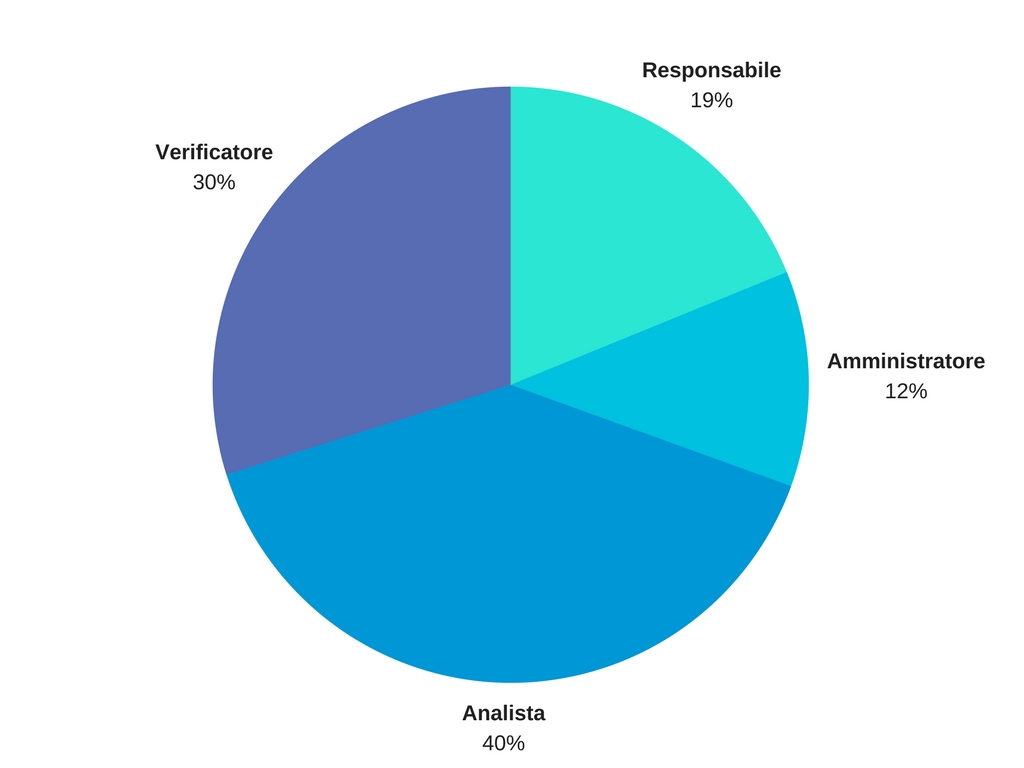
\includegraphics[width=0.9\textwidth]{images/CircolareAnalisiRequisitiDiMassima.jpg} 
				\caption{Diagramma circolare ripartizione ore per ruolo in Analisi dei Requisiti di Massima}
			\label{CircolareAnalisiRequisitiDiMassima}
			\end{figure}

			
			Come precedentemente detto nella sezione 3.1.2 di questo documento nel periodo di attesa dell'esito di questa attività ogni componente del grupo dovrà impegnare 10 ore in attività di approfondimento e studio delle tecnologie utili ai fini del profetto. Questo impegno non sarà rendicontato al proponente, nè ne sarà fornita una stima di costo in quanto non è assimilabile a nessun ruolo di progetto.
		
		\subsubsection{Analisi dei Requisiti di Dettaglio}
			\paragraph{Suddivisione lavoro}
			Nell'attività di \textit{Analisi dei Requisiti di Dettaglio} ciascun componente andrà a rivestire i seguenti ruoli:
			\begin{table}[H]
				\centering
				\begin{tabular}{|C{4cm}|C{0.6cm}|C{0.6cm}|C{0.6cm}|C{0.6cm}|C{0.6cm}|C{0.6cm}|C{3cm}|}
					\hlineB{3}
					\thead{Nominativo} &\thead{Re} &\thead{Am} &\thead{An}&\thead{Pt}&\thead{Pr}&\thead{Ve}&\thead{Ore totali}\\
					\hlineB{3}
					Paolo Eccher        & - & 3 & 3 & - & - & - & 6 \\
					Alberto Gallinaro   & - & - & 4 & - & - & 2 & 6 \\
					Giuseppe Merlino    & - & - & 4 & - & - & 3 & 7 \\
					Elia Montecchio     & - & - & 3 & - & - & 3 & 6 \\
					Lisa Parma          & 6 & - & - & - & - & - & 6 \\
					Francesco Parolini  & 4 & - & 2 & - & - & - & 6 \\
					Davide Zago         & - & - & 3 & - & - & 2 & 5 \\
					\textbf{Ore totali ruolo}  & \textbf{10} & \textbf{3} & \textbf{19} & \textbf{-} & \textbf{-} & \textbf{10} & \textbf{42} \\
					\hlineB{3}
				\end{tabular}
				\caption{Suddivisione del lavoro - \textit{Analisi dei Requisiti di Dettaglio}}
			\end{table}
			
			Tali dati sono raissunti nel seguente diagramma a barre:
			
			\textcolor{red}{METTERE DIAGRAMAM}

			\paragraph{Prospetto economico}
			Nello svolgimento di questa attività i costi sostenuti per ogni ruolo sono raissunti nella seguente tabella:
			\begin{table}[H]
			\centering
			\begin{tabular}{|p{4cm}|C{4cm}|C{4cm}|}
				\hlineB{3}
				
				\thead{Ruolo} &\thead{Ore previste} &\thead{Costo}\\
				\hlineB{3}			
				Responsabile & 10 & 300,00\euro \\
				\hline
				Amministratore& 3 & 60,00\euro \\
				\hline
				Analista & 19 & 475,00\euro \\
				\hline
				Progettista & - & 0\euro \\
				\hline
				Programmatore & - & 0\euro \\
				\hline
				Verificatore & 10 & 150,00\euro \\
				\hline
				\textbf{Ore totali} & \textbf{42} & \textbf{985.00 \euro} \\
				\hlineB{3}
			\end{tabular}
			\caption{Costi per ruolo \textit{Analisi dei Requisiti di Dettaglio}}
		\end{table}
		
		La ripartizione delle ore tra i vari ruoli è rappresentata graficamente tramite il seguente diagramma circolare:

			\begin{figure}[h] 
			\centering 
			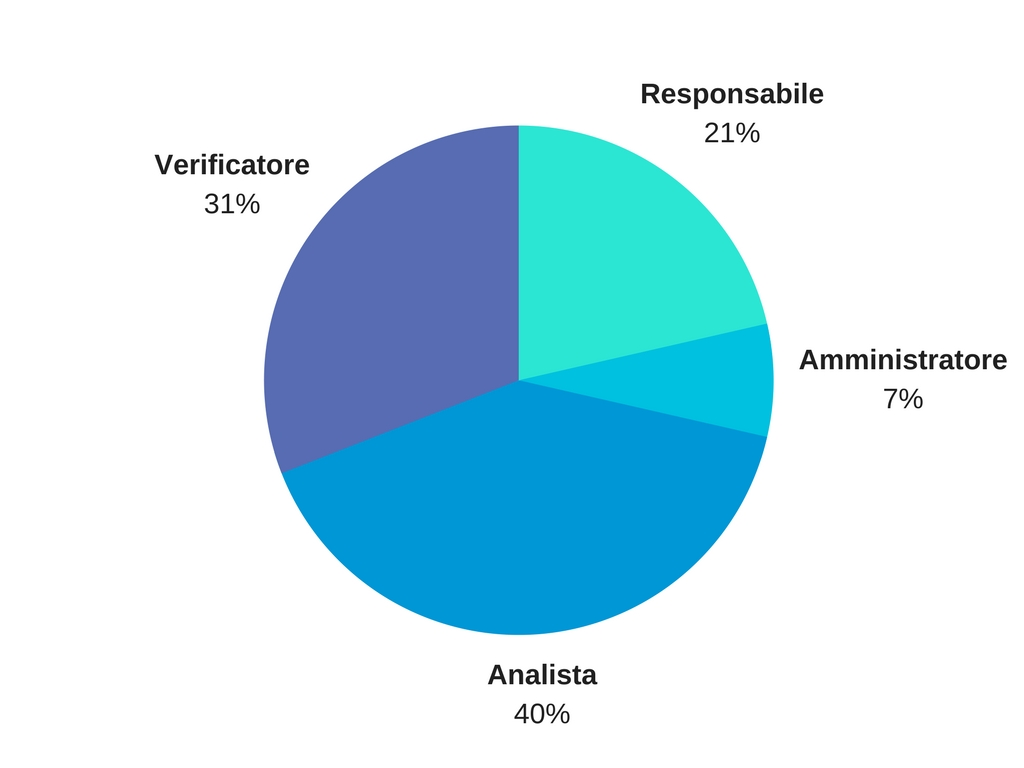
\includegraphics[width=0.9\textwidth]{images/CircolareAnalisiRequisitiDiDettaglio.jpg} 
			\caption{Diagramma circolare ripartizione ore per ruolo - \textit{Analisi dei Requisiti di Dettaglio}}
			\label{CircolareAnalisiRequisitiDiDettaglio}
			\end{figure}
		


		\subsubsection{Progettazione Architetturale}
			\paragraph{Suddivisione lavoro} \Spazio
				Nell'attività di \textit{Progettazione Architetturale} ciascun componente andrà a rivestire i seguenti ruoli:
				\begin{table}[H]
					\centering
					\begin{tabular}{|C{4.5cm}|C{0.7cm}|C{0.7cm}|C{0.7cm}|C{1cm}|C{0.7cm}|C{0.7cm}|C{3cm}|}
						\hlineB{3}
						\thead{Nominativo} &\thead{Re} &\thead{Am} &\thead{An}&\thead{Pt}&\thead{Pr}&\thead{Ve}&\thead{Ore totali}\\
						\hlineB{3}
						Paolo Eccher      & 6 & - & - & 14 & - & 6 & 26 \\
						Alberto Gallinaro & - & 3 & - & 17 & - & 5 & 25 \\
						Giuseppe Merlino  & - & - & - & 15 & - & 10 & 25 \\
						Elia Montecchio   & 3 & - & - & 12 & - & 10 & 25 \\
						Lisa Parma        & 1 & - & - & 16 & - & 9 & 26 \\
						Francesco Parolini& - & 5 & - & 10 & - & 10 & 25 \\
						Davide Zago       & - & - & - & 18 & - & 7 & 25 \\
						\textbf{Ore totali ruolo}  & \textbf{10} & \textbf{8} & \textbf{-} & \textbf{102} & \textbf{-} & \textbf{57} & \textbf{177} \\
						\hlineB{3}
					\end{tabular}
					\caption{Suddivisione del lavoro - \textit{Progettazione Architetturale}}
				\end{table}
				
			Tali dati sono riassunti graficamente nel seguente diagramma a barre:
			
			\textcolor{red}{METTERE DIAGRAMAM}
							
			\paragraph{Prospetto economico} \Spazio
			Nello svolgimento di questa attività i costi sostenuti per ogni ruolo sono riassunti nella seguente tabella:
			\begin{table}[H]
			\centering
			\begin{tabular}{|p{4cm}|C{4cm}|C{4cm}|}
				\hlineB{3}
				
				\thead{Ruolo} &\thead{Ore previste} &\thead{Costo}\\
				\hlineB{3}			
				Responsabile & 10 & 300,00\euro \\
				\hline
				Amministratore& 8 & 160,00\euro \\
				\hline
				Analista & - & 0\euro \\
				\hline
				Progettista & 102 & 2244,00\euro \\
				\hline
				Programmatore & - & 0\euro \\
				\hline
				Verificatore & 57 & 855,00\euro \\
				\hline
				\textbf{Ore totali} & \textbf{177} & \textbf{3.559.00 \euro} \\
				\hlineB{3}
			\end{tabular}
			\caption{Costi per ruolo - \textit{Progettazione Architetturale}}
		\end{table}
		
		La ripartizione delle ore tra i vari ruoli è rappresentata graficamente tramite il seguente diagramma circolare:
		
		\begin{figure}[h] 
			\centering 
			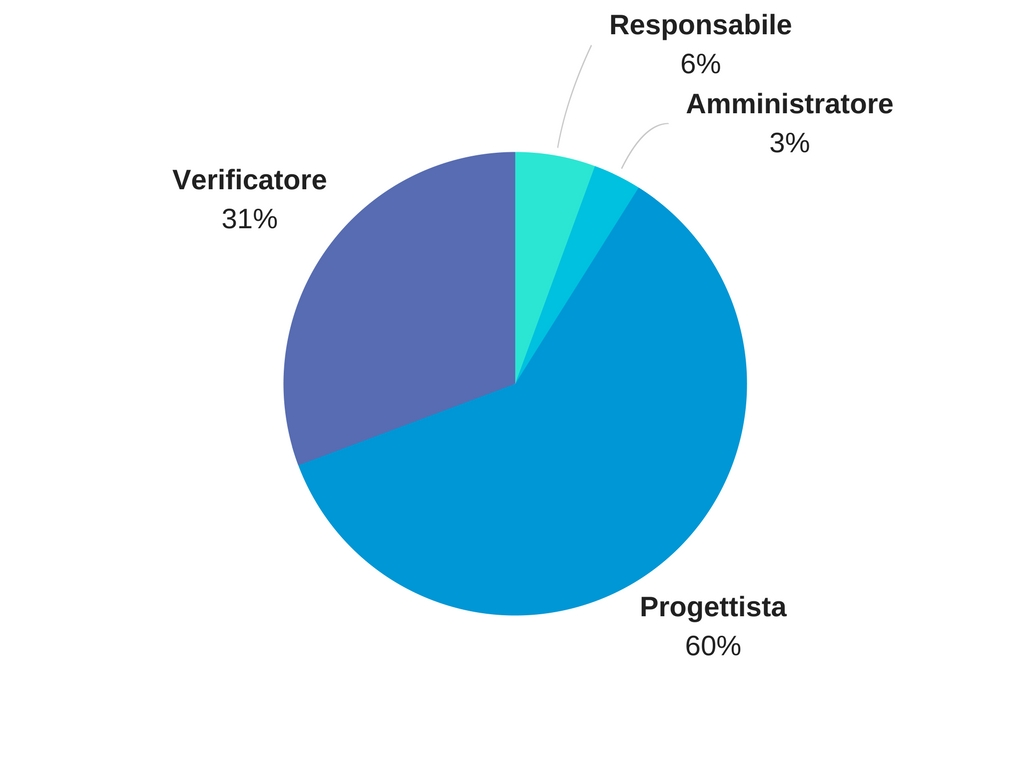
\includegraphics[width=0.9\textwidth]{images/CircolareProgettazioneArchitetturale.jpg} 
			\caption{Diagramma circolare ripartizione ore per ruolo in Progettazione Architetturale}
			\label{CircolareProgettazioneArchitetturale}
		\end{figure}		

		
		\subsubsection{Progettazione di Dettaglio}
			\paragraph{Suddivisione lavoro}
			Nell'attività di \textit{Progettazione di Dettaglio} ciascun componente andrà a rivestire i seguenti ruoli:
			
			\begin{table}[H]
				\centering
				\begin{tabular}{|C{4cm}|C{0.6cm}|C{0.6cm}|C{0.6cm}|C{0.6cm}|C{0.6cm}|C{0.6cm}|C{3cm}|}
					\hlineB{3}
					\thead{Nominativo} &\thead{Re} &\thead{Am} &\thead{An}&\thead{Pt}&\thead{Pr}&\thead{Ve}&\thead{Ore totali}\\
					\hlineB{3}
					Paolo Eccher      & - & - & - & 23 & - & - & 23 \\
					Alberto Gallinaro & 6 & - & - & 16 & - & 2 & 24 \\
					Giuseppe Merlino  & - & - & - & 2 & - & 20 & 22 \\
					Elia Montecchio   & 2 & - & - & - & - & 22 & 24 \\
					Lisa Parma        & - & 3 & - & 20 & - & - & 23 \\
					Francesco Parolini& - & - & - & 17 & - & 6 & 23 \\
					Davide Zago       & - & 4 & - & 14 & - & 5 & 23 \\
					\textbf{Ore totali ruolo}  & \textbf{8} & \textbf{7} & \textbf{-} & \textbf{92} & \textbf{-} & \textbf{55} & \textbf{162} \\
					\hlineB{3}
				\end{tabular}
				\caption{Suddivisione del lavoro - \textit{Progettazione di Dettaglio}}
			\end{table}
			
			Tali dati sono riassunti graficamente nel seguente diagramma a barre:
			
			\textcolor{red}{METTERE DIAGRAMAM}
			
			\paragraph{Prospetto economico} \Spazio
			Nello svolgimento di questa attività i costi sostenuti per ogni ruolo sono riassunti nella seguente tabella:
			\begin{table}[H]
			\centering
			\begin{tabular}{|p{4cm}|C{4cm}|C{4cm}|}
				\hlineB{3}
				
				\thead{Ruolo} &\thead{Ore previste} &\thead{Costo}\\
				\hlineB{3}			
				Responsabile & 8 & 240,00\euro \\
				\hline
				Amministratore& 7 & 140,00\euro \\
				\hline
				Analista & - & 0\euro \\
				\hline
				Progettista & 92 & 2.024,00\euro \\
				\hline
				Programmatore & - & 0\euro \\
				\hline
				Verificatore & 55 & 825,00\euro \\
				\hline
				\textbf{Ore totali} & \textbf{162} & \textbf{3.229,00 \euro} \\
				\hlineB{3}
			\end{tabular}
			\caption{Costi per ruolo - \textit{Progettazione di Dettaglio}}
		\end{table}
		
		La ripartizione delel ore tra i vari ruoli è rappresentata graficamente tramite il seguente diagramma circolare:
		
		\begin{figure}[h] 
			\centering 
			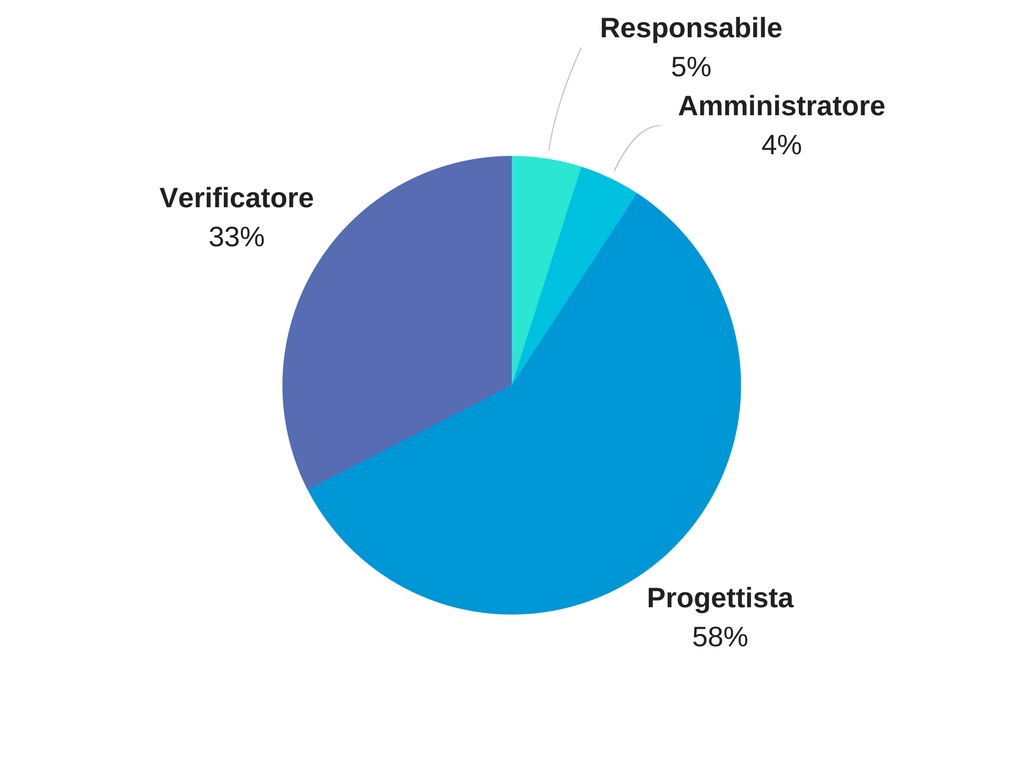
\includegraphics[width=0.9\textwidth]{images/CircolareProgettazioneDiDettaglio.jpg} 
			\caption{Diagramma circolare ripartizione ore per ruolo in Progettazione di Dettaglio}
			\label{CircolareProgettazioneDiDettaglio}
		\end{figure}		
		
		
		\subsubsection{Codifica}
			\paragraph{Suddivisione lavoro}
			Nell'attività di \textit{Codifica} ciascun componente andrà a rivestire i seguenti ruoli:
			\begin{table}[H]
				\centering
				\begin{tabular}{|C{4cm}|C{0.6cm}|C{0.6cm}|C{0.6cm}|C{0.6cm}|C{0.6cm}|C{0.6cm}|C{3cm}|}
					\hlineB{3}
					\thead{Nominativo} &\thead{Re} &\thead{Am} &\thead{An}&\thead{Pt}&\thead{Pr}&\thead{Ve}&\thead{Ore totali}\\
					\hlineB{3}
					Paolo Eccher      & - & - & - & 10 & 10 & 13 & 33 \\
					Alberto Gallinaro & 5 & - & - & 10 & 18 & - & 33 \\
					Giuseppe Merlino  & - & 6 & - & - & 28 & - & 34 \\
					Elia Montecchio   & - & - & - & - & 13 & 20 & 33 \\
					Lisa Parma        & - & - & - & - & 13 & 20 & 33 \\
					Francesco Parolini& - & - & - & 7 & 18 & 9 & 34 \\
					Davide Zago       & 6 & - & - & - & 20 & 8 & 34 \\
					\textbf{Ore totali ruolo}  & \textbf{11} & \textbf{6} & \textbf{-} & \textbf{27} & \textbf{120} & \textbf{70} & \textbf{234} \\
					\hlineB{3}
				\end{tabular}
				\caption{Suddivisione del lavoro - \textit{Codifica}}
			\end{table}
			
			Tali dai sono riassunti graficamente nel seguente diagramma a barre:
			
			\textcolor{red}{METTERE DIAGRAMAM}
			
			
			\paragraph{Prospetto economico} \Spazio
			Nello svolgimento di questa attività i costi sostenuti per ogni ruolo sono riassunti nella seguente tabella:
			\begin{table}[H]
				\centering
				\begin{tabular}{|p{4cm}|C{4cm}|C{4cm}|}
					\hlineB{3}
					
					\thead{Ruolo} &\thead{Ore previste} &\thead{Costo}\\
					\hlineB{3}			
					Responsabile & 11 & 330,00\euro \\
					\hline
					Amministratore& 6 & 120,00\euro \\
					\hline
					Analista & - & 0\euro \\
					\hline
					Progettista & 27 & 594,00\euro \\
					\hline
					Programmatore & 120 & 1.800,00\euro \\
					\hline
					Verificatore & 70 & 1.050,00\euro \\
					\hline
					\textbf{Ore totali} & \textbf{234} & \textbf{3.894,00 \euro} \\
					\hlineB{3}
				\end{tabular}
					\caption{Costi per ruolo - \textit{Codifica}}
			\end{table}
			
			La ripartizione delle ore tra i vari ruoli è rappresentata graficamente tramite il seguente diagramma circolare:

		\begin{figure}[H] 
			\centering 
			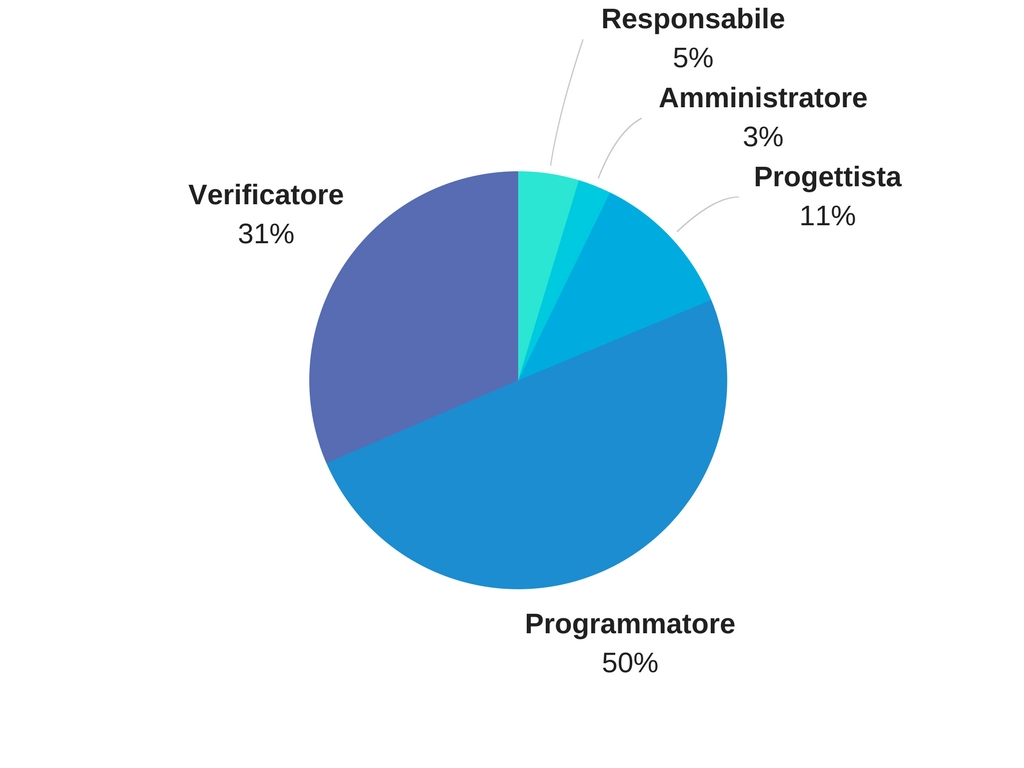
\includegraphics[width=0.9\textwidth]{images/CircolareCodifica.jpg} 
			\caption{Diagramma circolare ripartizione ore per ruolo in Codifica}
			\label{CircolareCodifica}
		\end{figure}
	
		\subsubsection{Validazione}
			\paragraph{Suddivisione lavoro} \Spazio
			Nell'attività di \textit{Validazione} ciascun componente del gruppo andrà a rivestire i seguenti ruoli:
			\begin{table}[H]
				\centering
				\begin{tabular}{|C{4cm}|C{0.6cm}|C{0.6cm}|C{0.6cm}|C{0.6cm}|C{0.6cm}|C{0.6cm}|C{3cm}|}
					\hlineB{3}
					\thead{Nominativo} &\thead{Re} &\thead{Am} &\thead{An}&\thead{Pt}&\thead{Pr}&\thead{Ve}&\thead{Ore totali}\\
					\hlineB{3}
					Paolo Eccher       & - & - & - & 2 & - & 12 & 14 \\
					Alberto Gallinaro  & - & 2 & - & - & - & 12 & 14 \\
					Giuseppe Merlino   & - & - & - & 3 & - & 12 & 15 \\
					Elia Montecchio    & - & - & - & 5 & - & 10 & 15 \\
					Lisa Parma         & - & - & - & 10 & - & 5 & 15 \\
					Francesco Parolini & - & - & - & - & - & 14 & 14 \\
					Davide Zago        & 6 & - & - & - & - & 9 & 15 \\
					\textbf{Ore totali ruolo}  & \textbf{6} & \textbf{2} & \textbf{-} & \textbf{20} & \textbf{-} & \textbf{74} & \textbf{102} \\
					\hlineB{3}
				\end{tabular}
				\caption{Suddivisione del lavoro - \textit{Validazione}}
			\end{table}
			
			Tali dati sono riassunti graficamente nel seguente diagramma a barre:
			
			\textcolor{red}{METTERE DIAGRAMAM}
			
			
			\paragraph{Prospetto economico}	\Spazio
			Nello svolgimento di questa attività i costi sostenuti per ogni ruolo sono riassunti nella seguente tabella:
			\begin{table}[H]
				\centering
				\begin{tabular}{|p{4cm}|C{4cm}|C{4cm}|}
					\hlineB{3}
					
					\thead{Ruolo} &\thead{Ore previste} &\thead{Costo}\\
					\hlineB{3}			
					Responsabile & 6 & 180,00\euro \\
					\hline
					Amministratore& 2 & 40,00\euro \\
					\hline
					Analista & - & 0\euro \\
					\hline
					Progettista & 20 & 404,00\euro \\
					\hline
					Programmatore & - & 0,00\euro \\
					\hline
					Verificatore & 74 & 1.110,00\euro \\
					\hline
					\textbf{Ore totali} & \textbf{102} & \textbf{1.734,00 \euro} \\
					\hlineB{3}
				\end{tabular}
				\caption{Costi per ruolo - \textit{Validazione}}
			\end{table}
			
			La ripartizione delle ore tra i vari ruoli è rappresentata graficamente tramite il seguente diagramma circolare:
			\textcolor{red}{METTERE DIAGRAMAM}		
				
				
								
	\subsection{Riepilogo}
		\subsubsection{Ore totali di investimento}
			\paragraph{Suddivisione lavoro} \Spazio
			Il totale delle ore investite, consideranto sia quelle rendicontate che quelle d'investimento non redicontate sono riassunte nella seguente tabella:
					\begin{table}[H]
			\centering
			\begin{tabular}{|C{4cm}|C{0.6cm}|C{0.6cm}|C{0.6cm}|C{0.6cm}|C{0.6cm}|C{0.6cm}|C{3cm}|}
				\hlineB{3}
				\thead{Nominativo} &\thead{Re} &\thead{Am} &\thead{An}&\thead{Pt}&\thead{Pr}&\thead{Ve}&\thead{Ore totali}\\
				\hlineB{3}
				Paolo Eccher 		& 6  & 6 & 16 & 49 & 10 & 37 & 124 \\
				Alberto Gallinaro 	& 11 & 5 & 20 & 43 & 18 & 27 & 124 \\
				Giuseppe Merlino 	& 13 & 6 & 6  & 20 & 28 & 52 & 125 \\
				Elia Montecchio 	& 5 & 3 & 15 & 17 & 13 & 71 & 124 \\
				Lisa Parma 			& 7 & 9 & 12 & 46 & 13 & 38 & 125 \\
				Francesco Parolini 	& 17 & 9 & 2 & 34 & 18 & 45 & 125 \\
				Davide Zago 		& 17 & 6 & 13 & 32 & 20 & 37 & 125 \\
				
				\textbf{Ore totali ruolo}  & \textbf{76} & \textbf{44} & \textbf{84} & \textbf{241} & \textbf{120} & \textbf{307} & \textbf{872} \\
				\hlineB{3}
			\end{tabular}
			\caption{Suddivisione del lavoro - Investimento totale }
			\end{table}
		
			Tali dati sono riassunti graficamente nel seguente diagramma a barre:
			
			\textcolor{red}{DIAGRAMAM}
			
			La ripartizione delle ore tra i vari ruoli è rappresentata graficamente 
			attraverso il seguente diagramma circolare:
			
			\textcolor{red}{DIAGRAMAM}
			
			\subsubsection{Ore Rendicontate}
			
			\paragraph{Suddivisione lavoro} \Spazio
			Le ore rendicontate sono riassunte nella seguente tabella:
			\begin{table}[H]
				\centering
				\begin{tabular}{|C{4cm}|C{0.6cm}|C{0.6cm}|C{0.6cm}|C{0.6cm}|C{0.6cm}|C{0.6cm}|C{3cm}|}
					\hlineB{3}
					\thead{Nominativo} &\thead{Re} &\thead{Am} &\thead{An}&\thead{Pt}&\thead{Pr}&\thead{Ve}&\thead{Ore totali}\\
					\hlineB{3}
					Paolo Eccher       & 4 & 3 & 4 & 49 & 10 & 35 & 105 \\
					Alberto Gallinaro  & 7 & 4 & 5 & 43 & 18 & 28 & 105 \\
					Giuseppe Merlino   & 8 & 4 & 0 & 20 & 28 & 45 & 105 \\
					Elia Montecchio    & 4 & 0 & 3 & 17 & 13 & 68 & 105 \\
					Lisa Parma         & 5 & 4 & 3 & 46 & 13 & 34 & 105 \\
					Francesco Parolini& 10 & 4 & 0 & 34 & 18 & 39 & 105 \\
					Davide Zago        & 8 & 5 & 2 & 32 & 20 & 38 & 105 \\
					\textbf{Ore totali ruolo}  & \textbf{46} & \textbf{24} & \textbf{17} & \textbf{241} & \textbf{120} & \textbf{287} & \textbf{735} \\
					\hlineB{3}
				\end{tabular}
				\caption{Suddivisione del lavoro - Ore rendicontate }
			\end{table}
			
			Tali dati sono riassunti graficamente nel seguente diagramma a barre:
			
			\textcolor{red}{DIAGRAMAM}
			
			\paragraph{Prospetto economico} \Spazio
			Il totale rendicontato dei costi sostenuti per ogni ruolo è riassunto nella seguente tabella:
			\begin{table}[H]
				\centering
				\begin{tabular}{|p{4cm}|C{4cm}|C{4cm}|}
					\hlineB{3}
					
					\thead{Ruolo} &\thead{Ore previste} &\thead{Costo}\\
					\hlineB{3}			
					Responsabile & 46 & 1.380,00\euro \\
					\hline
					Amministratore& 24 & 480,00\euro \\
					\hline
					Analista & 17 & 425,0\euro \\
					\hline
					Progettista & 241 & 5.302,00\euro \\
					\hline
					Programmatore & 120 & 1.800,00\euro \\
					\hline
					Verificatore & 287 & 4.305,00\euro \\
					\hline
					\textbf{Ore totali} & \textbf{735} & \textbf{13.692,00 \euro} \\
					\hlineB{3}
				\end{tabular}
				\caption{Costi per ruolo - Ore rendicontate}
			\end{table}
		
			La ripartizione delle ore tra i vari ruoli è rappresentata graficamente attraverso il seguente diagramma circolare:
		
			\textcolor{red}{DIAGRAMAM}
		
			
			\subsubsection{Conclusioni}
			
			Il costo totale preventivato per il progetto è 13.692,00 \euro.
